\documentclass{statsmsc}

\title{Statistics Research Project Title}
\author{FIRSTNAME LASTNAME}
\CID{01234567}
\supervisor{SUPERVISORNAME and COSUPERVISORNAME}
\date{1 May 2024}
%For today's date, use:
%\date{\today}
\logoimg{}

% THIS IS WHERE NEW COMMANDS CAN BE DEFINED

% commands below only used in the proof; otherwise can be deleted
\newcommand{\consta}{a}
\newcommand{\X}{X}
\newcommand{\EE}[1]{ \mathrm{E} [ #1 ] }
\newcommand{\inparenth}[1]{\left( #1 \right)}

\usepackage{xcolor}
\usepackage{hyperref}
\hypersetup{
    colorlinks,
    linkcolor={blue!50!black},
    citecolor={blue!50!black},
    urlcolor={blue!50!black}
}


\begin{document}

% Generates the Title Page
\maketitle

% Generates plagiarism declaration
\declarationname{STUDENT'S NAME}
\declarationdate{DATE}
\declaration 

\begin{acknowledgements}
    In the acknowledgments, you should account for anyone who supported you during your research. This could include family, your research peer group, other students, research group members, your supervisor, data providers, external partners, any computing service used, any financial support. 
    
    If your research peer group, other students, research group members, or your supervisors made substantive contributions towards your report -- e.g. they identified suitable methods, provided code or contributed a sub-analysis -- you must acknowledge their precise contribution here.
\end{acknowledgements}

%=================================================================
% VERY IMPORTANT
% This command switches from Roman to Arabic numbering for main part of report. Do not modify.
\mainmatter
%=================================================================


\begin{abstract}
    Abstracts should be no longer than 300 words, and similar in style to a general science or statistics research paper.
\end{abstract}

%===============================================================
%
% Students please remove the General tips when submitting your report
%
%===============================================================
\paragraph{General tips.} Your research report will be judged on the quality of the work it describes according to the Marking Criteria shared with you. 
When writing your research report you may assume that the reader is familiar with the four core modules of the MSc in statistics. Any additional other material should be explained to the reader, providing suitable references. See Section~\ref{sec:referencing} for more details. For example, you should avoid writing up in detail statistical methods discussed in one of the four core modules, but instead you should briefly present such methods and add appropriate references. More advanced methods or methods discussed in one of the elective modules should be described in more detail and referenced appropriately. 

Your report must be presented within this template and be at most 35 pages in length, as counted by the Arabic page numerals (1,2,3…). This limit includes all figures and tables presented in the main text, as well as the Endmatter and References sections. This is approximately equivalent to a limit of 15,000 words. Shorter submissions may be graded highly, while excess length disproportionate to the content may be penalised.


Before submitting the research project, make sure you read the report in its entirety. There should be no half-finished sentences. All mathematical symbols should be defined. Use a spell-checker.

You will have to submit your report electronically in PDF format through the virtual learning environment (Blackboard). Please name this file in the following format: “CID-Surname-Firstname-Report.pdf”. Your report will be checked for plagiarism via online plagiarism detection services (e.g. Turnitin). 

Note the report submission deadline is a very hard deadline since the assessment process has then to be completed on a very short timescale.

\section{Introduction}

\paragraph{Tips for the Introduction.} This is where you describe the topic and the research objectives of your project. 

You should attempt to set your work in the context of other work previously done in the field. Convey the background of your research referencing earlier work as appropriate. Define core terms. Include background and context, and focus as appropriate on the wider statistical context. Aim to demonstrate that you can confidently describe your project within a broader context of statistical research, as well as scientific research, that goes well beyond the more narrow topic of your project.


The introduction needs to demonstrate that you are aware of what you are doing, and how it relates to other work that should be properly referenced. 

Clearly point out your main contributions at the end of the introduction, and provide an overview how the rest of your report is structured and links together. 

Aim for approximately 1.5-3 pages, similar in style to a general science or statistics research paper.\footnote{Tip: If you choose to use footnotes, do so sparingly.}.





\section{Methods}\label{sec:methods}


\paragraph{Tips for the Methods section.} In general, you may structure the main body of your report in a form that suits your project best. We recommend to start with a substantial Methods section that includes, as in a research paper, a description of the following:
\begin{itemize}
    \item Key definitions and setting using mathematical notation. Any terminology related to the topic/data needs to be clearly presented and explained to the reader.
    \item Any data used in the project should be clearly explained in sufficient detail in the Methods section so that readers can follow the rest of your report without the need to consult an other report or any of your references.
    \item If in the project you have generated simulated data, a clear presentation of the generative procedure needs to be included. 
    \item Background statistical work using mathematical notation.
    \item All maths should be presented in inline or display formulas with appropriate referencing. For example, use $\exp(x)$ not exp(x) and $\sin(\theta)$ not $sin(\theta)$ or sin($\theta$). Display formulas should be numbered using the equation environment if they are referenced in the main text. Display equation blocks should be numbered using the subequations environment:
\begin{subequations}\label{eq:Y}
    \begin{align}
        Y & = 1 + Z \label{eq:Y1} \\ 
        Z & \sim \mathcal{N}(0,1) \label{eq:Y2},
    \end{align}
\end{subequations}
    so that you can reference~\eqref{eq:Y}, ~\eqref{eq:Y1}, and ~\eqref{eq:Y2}.
    \item If your main findings are of an applied nature, you may prefer to describe any new/original statistical procedures or models here. Include the key derivations and proofs if there are any, and any supplementary derivations in the appendix. Clearly highlight your contribution relative to existing work. 
    \item If your main findings are of a theoretical nature, you may prefer to describe any new/original statistical procedures or models in the Results section.
    \item Structure your Methods section using LaTeX   subsections and reference them using labels.
    \item Aim for approximately 8-15 pages, similar in style to a general science or statistics research paper.
\end{itemize}


\subsection{My Methods subsection}\label{subsec:my_subsec}

This text is in Subsection~\ref{subsec:my_subsec}, which is a part of Section~\ref{sec:methods}.

\subsubsection{My subsubsection}
If needed, subsections can also have subsubsections within them. Keep subsections and subsubsections numbered, which will help us to reference them.


\paragraph{Paragraphs.} In the rare event that you need a more deeply nested structure within a subsubsection, the \texttt{\textbackslash paragraph\{\}} command can be useful. 

\section{Results}

\paragraph{Tips for the Results section.} 

\begin{itemize}
    \item If your main findings are of a theoretical nature, you may prefer to describe any new/original statistical procedures or models in the Results section.
    \item Describe your findings concisely and precisely using scientific language. 
    \item Include sound interpretations and explanations wherever possible to demonstrate your original and clear statistical thought process. 
    \item Use figures and tables to support your main arguments, which should include a caption describing, e.g., what is shown on the $x-$ and $y$-axis or in the rows and columns. Summarise the main finding or headline numbers in the main text, including references to Figures and Tables as needed. Do not report all numbers shown in a figure or table.
    \item Include references to previous work as needed. 
    \item Structure your Results section into numbered Subsections and Subsubsections as needed, and feel free to reference these throughout.
    \item Aim for approximately 5-15 pages, similar in style to a general science or statistics research paper.
\end{itemize}

\section{Discussion}

\paragraph{Tips for the Discussion section.} 

\begin{itemize}
    \item Begin your Discussion with a summary and the main findings of your research in 2-5 sentences.
    \item Describe the implications of your main findings in the context of existing work concisely and precisely using scientific language. 
    \item Describe the limitations in your statistical methods and your main findings. Be honest about the limitations in your approach, and substantiate what could have been done differently as needed. Explain if your main findings are robust or sensitive to these limitations.
    \item Avoid Subsections and Subsubsections in the Discussion.
    \item In the last paragraph, conclude your report with a pitch using plain language that summarises the key implications of your research in the context of previous work. Write this last paragraph for the Imperial Press Office or journalists as audience.
    \item Aim for approximately 1-3 pages, similar in style to a general science or statistics research paper.
\end{itemize}

\section{Endmatter} \label{sec:endmatter}

\paragraph{Tips for the Endmatter section.} 

\begin{itemize}
    \item Include a data availability statement. Examiners must be able to reproduce your analyses on all the data investigated as would be the case during peer review of a research paper.
    \item Include a reproducibility statement, including the URL under which your code can be found. Except in very rare circumstances, your code should be freely and publicly available under a \href{https://creativecommons.org/licenses/by/4.0/deed.en}{CC-BY-4.0} license. Examiners must be able to see your code, and they must be able to run your code.
\end{itemize}

%=========================================================
%
%
%
% Students should not edit below here 
%
%
%
%=========================================================

%=========================================================
%% Create bibliography
%
% - Add your references by modifying the file `refs.bib`
%
%=========================================================

\clearpage

%%References part of the main text
% References: modify the file refs.bib
\bibliographystyle{apalike}
\bibliography{refs}

\clearpage

%=========================================================
%% Create supplementary material 
%
%
% - Providing supplementary materials to your report is voluntary and will not normally be read by your examiners.
% - If you wish to include supplementary materials, add these by modifying the file 
%   `supplementary.tex`
% - otherwise deactive the include command below
%
%
%=========================================================

%% reset page counter and start appendix pages numbering
\pagenumbering{arabic}
\renewcommand*{\thepage}{Supplementary Material Page \arabic{page}}
\renewcommand{\thesection}{\Alph{section}}
%% Supplementary Material goes here
\appendix
\pagebreak

\section{Supplementary Materials}

\paragraph{Tips for the Supplement.} Please note that the Supplementary Material is not normally read by your examiners. Include material that you might like to include for your own reference, for reference of others beyond your examiners, or as backup to your thesis in case of further discussion.

Here, we use the Supplement to provide further tips on writing your thesis.

\section{Figures}\label{sec:figuresection}

\paragraph{Tips for the Figures.} It is better to create figures in a vector-based format, such as PDF. For plots with very many elements these vector-based graphics can become large and slow to load. In these cases a high-resolution bitmap graphic, such as a png, is preferred. 

Remember to make fonts in figures large enough to be read once the plots are embedded in the report (compare the two plots within Figure~\ref{fig:axis-label-example}). You may need to make multiple versions of the same figure if you plan to use it in your report, poster and presentation.

All figures must be referenced in the main text of the report, in the order that they are referenced.

\begin{figure}[htbp]
    \centering
    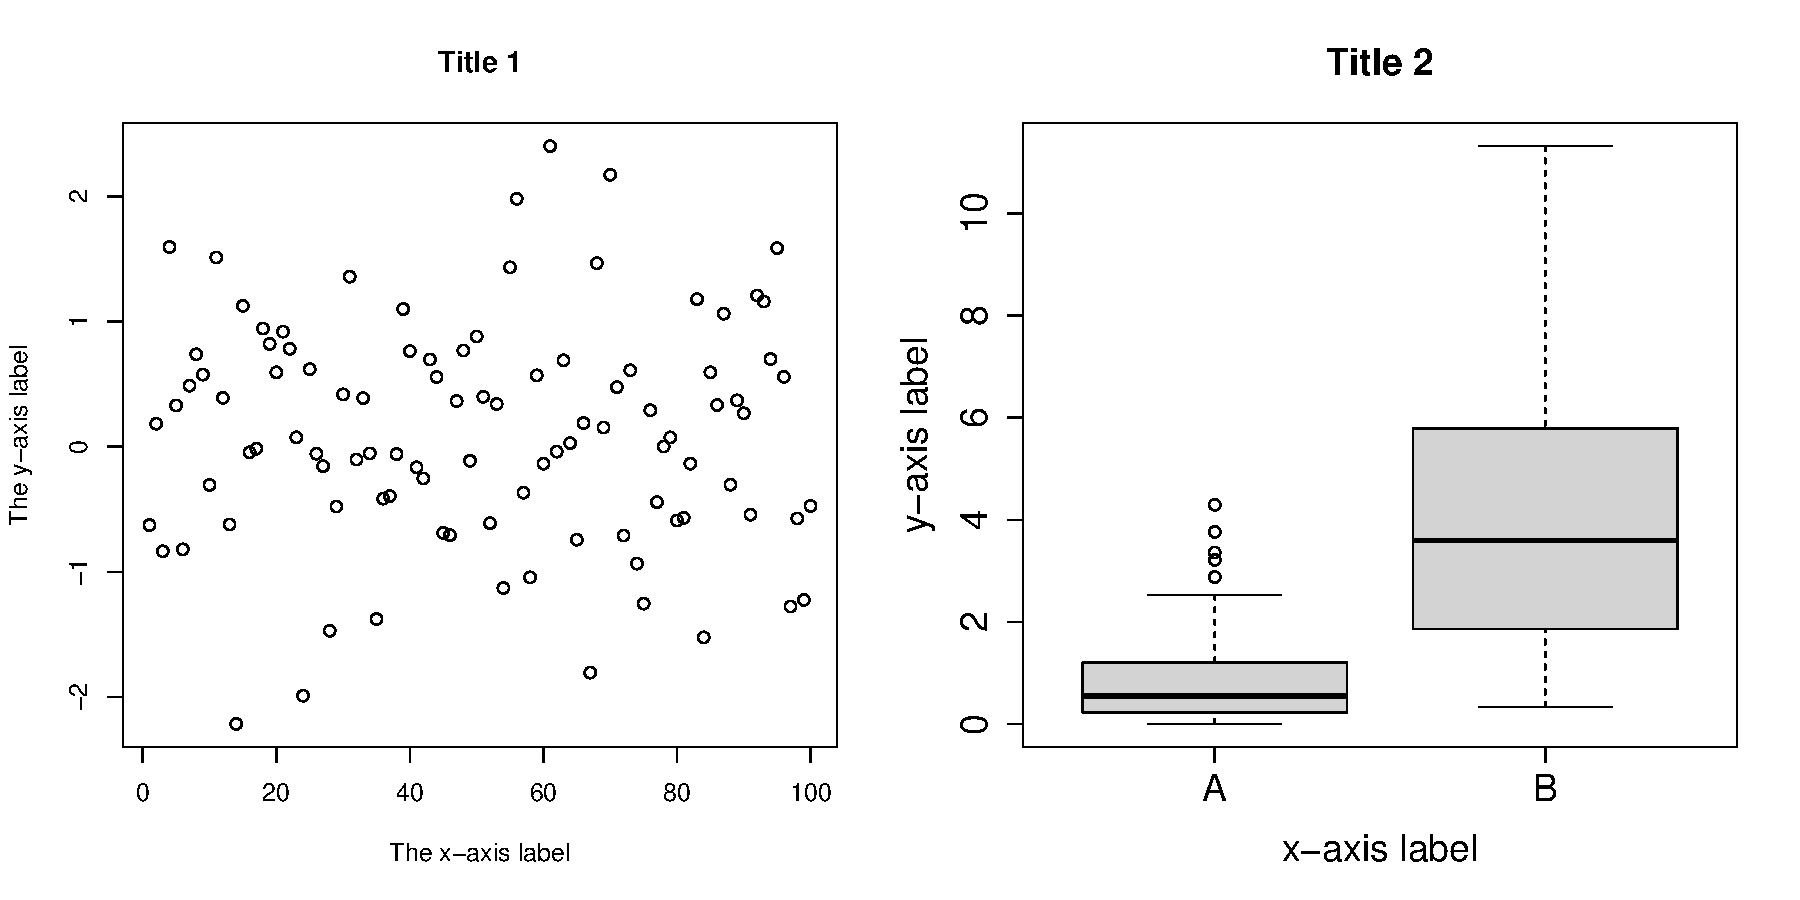
\includegraphics[width=0.9\textwidth]{images/fig1.pdf}
    \caption{An example scatterplot (left) and box plot (right).}
    \label{fig:axis-label-example}
\end{figure}

\section{Tables}\label{sec:tablesection}

\paragraph{Tips for the Tables.} Tables can be a useful way of displaying summary statistics. An example of a simple table is presented as Table~\ref{tab:normal}. All tables must be referenced in the main text of the report, in the order that they are referenced.

\begin{table}[ht]
\centering
\begin{tabular}{rr}
  \hline
    $z$& $\textrm{P}(Z < z)$ \\
  \hline
    1.281& 0.900\\
    1.645& 0.950\\
    1.960& 0.975\\
    2.326& 0.990 \\
    2.576& 0.995 \\
   \hline
\end{tabular}
    \caption{Partial table showing values of $z$ for $\textrm{P}(Z < z)$, 
    where $Z$ has a standard normal distribution.}
    \label{tab:normal}
\end{table}



\section{Referencing sources, sections and items} \label{sec:referencing}

\subsection{Referencing external sources}

You should give attribution to the academic books and articles that you draw from and build upon in your research report. You must give full attribution if and how you used generational AI during your research, referencing its use as outlined in our Guidance to using generational AI on the MSc in Statistics. You should use inline or parenthetical references to these sources. For example, a good book on the bootstrap is \cite{efrontib}, although the idea appeared in an earlier paper \citep{efron1979}.

Note that to make the references appear, you will need to compile the bibtex, otherwise you may just see question marks where the references should be. The small selection of example bibtex references used in this template are provided in the file \texttt{refs.bib}. These should be replaced with your own bibtex entries.
 
\subsection{Referencing elements of your report}

You might also want to cross reference results or claims from another part of your report such a as a section, result or equation. This is done by assigning a \texttt{\textbackslash label\{\}} to the item you wish to cross-reference and then using that label within \texttt{\textbackslash ref\{\}}. For example, Theorem~\ref{thm:variance-mse-relation} is proved in Section~\ref{sec:defnthms}. When referencing displayed mathematics, use \texttt{\textbackslash eqref\{\}}. As an example, see 
Equation~\eqref{eqn:variance-mse-relation}.

\subsubsection{Labelling tables and figures}

It is important that the label command
\texttt{\textbackslash label\{LABELNAME\}} comes \textbf{after} the caption command.
See Table~\ref{tab:normal} and Figure~\ref{fig:axis-label-example} as examples of this.

\subsection{Quoting sources}
If you wish to quote a source, be sure to use quotation marks and cite the
reference. The \texttt{\textbackslash{usequote}} command is useful here:

\usequote{It was the best of times, it was the worst of times, it was the age of wisdom, it was the age of foolishness, it was the epoch of belief, it was the epoch of incredulity, it was the season of Light, it was the season of Darkness, it was the spring of hope, it was the winter of despair, we had everything before us, we had nothing before us, we were all going direct to Heaven, we were all going direct the other way - in short, the period was so far like the present period, that some of its noisiest authorities insisted on its being received, for good or for evil, in the superlative degree of comparison only.} \citep{dickens1859}

\section{Definitions, theorems and examples}
\label{sec:defnthms}

The following environments are supported:
Definition, Theorem, Proof, Proposition, Lemma, Remark, Example.

\begin{definition} \label{defn:variance}
    The \textbf{variance} of a random variable $X$ is defined as
    \begin{equation} \label{eqn:variance-definition}
        \mathrm{Var}(X) = \mathrm{E}[(X - \mathrm{E}[X])^2].
    \end{equation}
\end{definition}

\begin{theorem} \label{thm:variance-mse-relation}
Given a random variable $X$, over all values $a \in \mathbb{R}$, 
\begin{equation}
    \min_{a \in \mathbb{R}} \mathrm{E}[(X - a)^2] 
    = \mathrm{E}[(X - \mathrm{E}[X])^2].
    \label{eqn:variance-mse-relation}
\end{equation}
\end{theorem}

\begin{proof}   
    Starting with the left-hand side of Equation~\eqref{eqn:variance-mse-relation},
\begin{align}
% Example of using \newcommands; see above
\EE{ \inparenth{\X - \consta}^2 } 
&=  \EE{  \inparenth{\X - \EE{\X} + \EE{\X} - \consta}^2 } 
    \nonumber \\
&=  \EE{  \inparenth{ \X - \EE{\X} }^2 } 
    + 2 \EE{ \inparenth{ \X - \EE{\X} } \inparenth{ \EE{\X} - \consta} } +  
  \EE{ \inparenth{ \EE{\X} - \consta}^2  }    
    \nonumber \\
&=  \EE{  \inparenth{ \X - \EE{\X} }^2 } +  \inparenth{ \EE{\X} - \consta}^2
    \nonumber \\
& \geq \EE{  \inparenth{ \X - \EE{\X} }^2 },  
\nonumber 
\end{align}
since $\EE{\X}$ is a real number and $\inparenth{ \EE{\X} - \consta}^2 \geq 0$,
and the third line follows from linearity of expectation:
%
\begin{align}
    \EE{ \inparenth{ \X - \EE{\X} } \inparenth{ \EE{\X} - \consta} }
    =
    \inparenth{ \EE{\X} - \consta} \EE{ \inparenth{ \X - \EE{\X} } }
    =
    \inparenth{ \EE{\X} - \consta}  \inparenth{\EE{ \X} - \EE{\X} } 
    =
    0,
    \nonumber
\end{align}
%
since $\EE{\EE{\X}} = \EE{\X}$, which proves the result.
\end{proof}

\begin{remark}
    This theorem shows that that the minimum of the quantity
    $\mathrm{E}[(X - a)^2]$ is equal to $\mathrm{Var}(X)$.
    In some sense, this makes the variance a natural measure of dispersion if 
    we are taking the metric to be the squared deviation of $X$.
\end{remark}


\begin{lemma}[Stein's Lemma]
    Let $X \sim \mathrm{N}(\mu, \sigma^2)$, and let $g$ be a differentiable 
    function satisfying $\mathrm{E}[|g'(X)|] < \infty$. Then
    \begin{equation}
        \mathrm{E}[g(X)(X-\mu)] = \sigma^2 \mathrm{E}[g'(X)].
        \nonumber
    \end{equation}
\end{lemma}

\begin{proposition}[Popoviciu's inequality]
    Suppose that the random variable $X$ is known to only take values in the 
    bounded range $[a, b]$. Then  
    \begin{align}
        \mathrm{Var}[X] \leq \dfrac{(b-a)^2}{4}.
        \nonumber
    \end{align}
\end{proposition}

\begin{example}
    Suppose $X \sim \mathrm{Bern} (p)$, for some $p \in [0,1]$. Then, 
    since $X \in \{0, 1\}$, $X$ is bounded between $0$ and $1$ and so
    $\mathrm{Var}[X] \leq \tfrac{1}{4}$.
\end{example}

Note that Equations~\eqref{eqn:variance-definition} and \eqref{eqn:variance-mse-relation} are numbered because they are referred to elsewhere in the main text. All other equations are unnumbered. 

Each of these environments may be labelled and referenced as with sections. For example, we might discuss Definition~\ref{defn:variance} or Theorem~\ref{thm:variance-mse-relation} in this paragraph. 

%=========================================================


\end{document}
